\documentclass[12pt,a5paper]{article}

\usepackage[T1]{fontenc} % font encoding, lubab õ tähte kasutada
\usepackage[utf8]{inputenc} % oleme siiski 21. sajandis, vajadusel on ka olemas utf8x
\usepackage{lmodern} % lmodern ja micrtype käivad käsikäes, teeb teksti ilusamaks
\usepackage{microtype}
\usepackage[estonian]{babel} % eesti keele poolitamisreeglid jpm
\usepackage[per = fraction, expproduct=cdot, decimalsymbol=comma]{siunitx} % http://www.bakoma-tex.com/doc/latex/siunitx/siunitx.pdf
\usepackage{graphicx} 
\usepackage{wrapfig}
\usepackage{epstopdf} %minul on vaja, et .eps pilte saada
\usepackage{circuitikz}
\usepackage{tikz}
\usepackage{xcolor}
\usepackage{enumitem}
%paneme kõik mõõdud paika
\topmargin=-2.9cm \textheight=18.8cm \textwidth=12.77cm
\oddsidemargin=-1.5cm  \evensidemargin=-1.5cm
\setlength{\parindent}{0pt} \setlength{\parskip}{4pt} \sloppy
\relpenalty=10000 \binoppenalty=10000 % Tekstisisestes valemites reavahetusi ärgu olgu
\pagestyle{empty} % ilma leheküljenumbrita
\newcommand{\numb}[1]{\vspace{5pt}\textbf{\large #1}}
\newcommand{\nimi}[1]{(\textsl{\small #1})}
\newcommand{\punktid}[1]{(\emph{#1~p.})}
\newcounter{ylesanne}
\newcommand{\yl}[1]{\addtocounter{ylesanne}{1}\numb{\theylesanne.} \nimi{#1} \newblock{}}
\newcommand{\autor}[1]{\emph{ Autor: #1}}


%  Abifunktsioon elektriskeemi joonise jaoks


\begin{document}

\begin{center}
\textbf{\Large Eesti koolinoorte 67. füüsikaolümpiaad} \vspace{2pt}

\emph{18. jaanuar 2020. a. Piirkondlik voor.}

\emph{Gümnaasiumi ülesanded (10. - 12. klass)}

\end{center}

\yl{SAUN} Juhan ja Peeter on saunas ning Juhan viskab kuumale kivikerisele külma vett temperatuuriga $\SI{10}{\celsius}$. Peeter väidab, et Juhan jahutab kerise niimoodi ära ja ütleb Juhanile, et ta viskaks külma vee asemel kuuma vett temperatuuriga $\SI{80}{\celsius}$. Juhan aga väidab vastu, et külma ja kuuma vee kasutamisel ei ole erilist vahet (kerise jahtumise erinevus on väiksem kui 10\%). Kui palju väheneb kerise temperatuur kummalgi juhul, kui visata sinna $V=\SI{200}{cm^3}$ vett? Kas Juhanil on õigus? Vee tihedus $\rho=\SI{1000}{kg/m^3}$, erisoojus $c_v=\SI{4200}{J/(kg\cdot\celsius)}$ ja aurustumissoojus $L=\SI{2300}{kJ/kg}$. Kerisekivide erisoojus $c_k=\SI{700}{J/(kg\cdot\celsius)}$ ja kogumass $M=\SI{100}{kg}$. Võib eeldada, et keris on piisavalt kuum ja kogu vesi aurustub ära. \punktid{6}

\yl{KARUSSELL} Juku läheb lõbustusparki ja märkab tiirlevat karusselli. Karussell koosneb ringikujulisest horisontaalsest kettast, mille küljes ripuvad kettide otsas lõbusõitjad. Juku märkab, et kinnitusketid moodustavad karusselli täiskiirusega pöörlemisel vertikaali suhtes nurga $\theta = \SI{60}{\degree}$.  Leia lõbusõitjate joonkiirus, kui karussell pööreleb täiskiirusel. Mitu tiiru minutis teeb karussell täiskiirusega pööreldes? Karusselli ketta raadius $R=\SI{10}{m}$, kettide pikkus $l=\SI{2}{m}$, raskuskiirendus $g=\SI{9,8}{m / s^2}$. Kettide kaalu mitte arvestada. \punktid{8}


\begin{wrapfigure}[10]{r}{0.3\textwidth}
    \vspace{-30pt}
	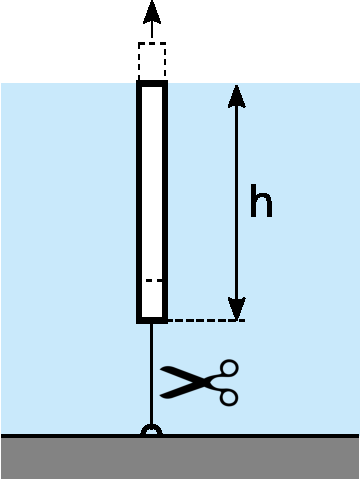
\includegraphics[width=0.3\textwidth]{hyppav_silinder.pdf}
\end{wrapfigure}


\yl{HÜPPAV SILINDER}
Peenike seest tühi silinder on nööriga kinnitatud veega täidetud basseini põhja nii, nagu näidatud joonisel. 
Silindri ülemine ots asub veepinnal. Nöör lõigatakse läbi ja silinder hakkab ülespoole liikuma ning hüppab veest välja. Kui kõrgele õhku tõuseb silindri alumine ots veepinnast maksimaalselt? Eeldage, et veest täielikult väljumise hetkel läheb 50\% silindri kineetilisest energiast kaduma silindri ja veepinna vastastikmõju tõttu. Muude keskkonna takistusjõududega ei pea arvestama.
Silindri mass $m = \SI{30}{g}$, raadius $r = \SI{1}{cm}$ ja kõrgus $h = \SI{0.5}{m}$. Vee tihedus $\rho_v=\SI{1000}{kg/m^3}$. \punktid{8}


\begin{wrapfigure}[9]{r}{0.5\textwidth}
\hspace{10pt}
\begin{circuitikz}[scale=0.5]
  \tikzset{
    declare function={
      atan3(\a,\b)=ifthenelse(atan2(0,1)==90, atan2(\a,\b), atan2(\b,\a));},
    kinky cross radius/.initial=+.3cm,
    @kinky cross/.initial=+, kinky crosses/.is choice,
    kinky crosses/left/.style={@kinky cross=-},kinky crosses/right/.style={@kinky cross=+},
    kinky cross/.style args={(#1)--(#2)}{
      to path={
        let \p{@kc@}=($(\tikztotarget)-(\tikztostart)$),
            \n{@kc@}={atan3(\p{@kc@})+180} in
        -- ($(intersection of \tikztostart--{\tikztotarget} and #1--#2)!%
               \pgfkeysvalueof{/tikz/kinky cross radius}!(\tikztostart)$)
        arc [ radius     =\pgfkeysvalueof{/tikz/kinky cross radius},
              start angle=\n{@kc@},
              delta angle=\pgfkeysvalueof{/tikz/@kinky cross}180 ]
        -- (\tikztotarget)}}}
  \draw (0,0) to[short, *-*] (0,0) to[european resistor] (0,4) to[short, *-*] (0,4)
  to[european resistor] (0,8) to[short, *-*,l=1] (0,8) to[european resistor] (4,8)
  to[short, *-*] (4,8) to[european resistor] (8,8) to[short, *-*] (8,8) to[european resistor] (8,4) to[short, *-*] (8,4) to[european resistor] (8,0) to[short, *-*,l_=2] (8,0) to[european resistor] (4,0) to[short, *-*] (4,0) to[european resistor] (0,0);

  \node (a) at (-0.125,4) {};
  \node (b) at (8.125,4) {};
  \node (c) at (4,8.125) {};
  \node (d) at (4,-0.125) {};


  \draw (c) -- (d);
  \draw (a) to [kinky cross=(c)--(d), kinky crosses=left] (b);
  \end{circuitikz}
\end{wrapfigure}

\yl{ELEKTRIRUUT} Leidke takistus punktide 1 ja 2 vahel (vt. joonis). Kõigi takistite takistus on $R$. \punktid{8}


\yl{PURILENNUK} Purilennuk veeti tuulevaiksel päeval puksiirköiega propellerlennuki järel kõrguseni $h = \SI{2000}{m}$ ja lasti seejärel lahti, mille tulemusel hakkas see ühtlase kiirusega maapinna poole liuglema. Kui suur on purilennuki maksimaalne lennukaugus lahtilaskmispunktist piki maapinda? Purilennuki mass koos piloodiga oli $m = \SI{500}{kg}$. Enne lahtilaskmist ühtlase kiirusega horisontaalselt lennates oli puksiirköies tekkiv tõmbejõud $T = \SI{120}{N}$ (puksiirköis oli siis samuti horisontaalne). Raskuskiirendus $g = \SI{9.8}{m/s^2}$. Võib eeldada, et purilennukile mõjuva aerodünaamilise tõstejõu ja õhutakistuse suhe $F_L/F_D$ on pukseerimisel ja vabal liuglemisel ühesugune. Aerodünaamiline tõstejõud $F_L$ on definitsiooni kohaselt risti lennuki kiirusvektoriga õhu suhtes ja õhutakistus $F_D$ on piki antud kiirusvektorit. \punktid{8}


\yl{KELL} Seinakellal on minuti ja tunniosuti, mis kaaluvad vastavalt
$m_1=\SI{5}{\gram}$ ja $m_2=\SI{25}{\gram}$, mille pikkused on vastavalt
$L_1=\SI{15}{\centi\meter}$ ja $L_2=\SI{10}{\centi\meter}$ ning mille otspunktid
on kinnitatud kella keskpunkti. Kella vooluallikas on tühjenemas ning täpselt kell kuus annab see maksimaalselt voolu $I=\SI{1}{\milli\ampere}$ pingel
$V=\SI{5}{\volt}$. Elektrienergiast jõuab osutiteni mehaaniline energia
kasuteguriga $\eta=0.3$. Leia minuti täpsusega aeg, mil kell jääb seisma. \punktid{10}

\yl{JÄLLE SAUNA!} Sauna leiliruumis on õhu temperatuur $t_0=\SI{80}\celsius$ ja leiliruumi ruumala $V=\SI{10}{m^3}$. Kerisele visati $m=\SI{200}g$ vett, mis paari sekundi jooksul kõik ära aurustus. Kui palju muutus õhu temperatuur leiliruumis? Eeldada, et tekkinud aur segunes täielikult leiliruumi õhuga ja rõhk leiliruumis püsis võrdne välise õhurõhuga tänu õhu liikimisele läbi uksealuse pilu. Õhurõhk $p_0=\SI{1e5}{Pa}$, vee molaarmass  $\mu_w=\SI{18}{g/mol}$, ühe mooli õhu soojusmahtuvus konstantsel ruumalal $c_a=\frac 53 R$ ja ühe mooli veeauru soojusmahtuvus konstantsel ruumalal $c_w=2R$. \punktid{10}


\yl{DIOODID} Dioodide tootmisel fluktueeruvad nende parameetrid märkimisväärselt. Olgu meil kaks valgusdioodi, mille pinged erinevad samasuguse tugevusega voolu korral 2\% võrra; nende dioodide voolu-pinge tunnusjooned on toodud juuresoleval joonisel punase ja sinise kõverana. Nende dioodide toitmiseks kasutatakse konstantse voolu allikat, mille väljundvool püsib konstantselt võrdne $I_0=\SI{2.7}A$ seni kuni väljundpinge pole suurem kui $\SI 4V$. Dioodid ühendatakse paralleelühenduses vooluallika klemmide külge; mitme protsendi võrra erinevad nende tarbitavad võimsused? \punktid{10}

\begin{wrapfigure}[12]{r}{0.5\textwidth}
\vspace{-15pt}
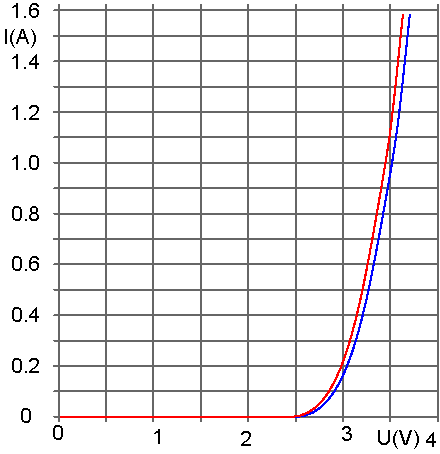
\includegraphics[width = 0.45\textwidth]{2dioodi-vi}
\end{wrapfigure}



\yl{LAENGUD MAGNETVÄLJAS} Ruumipiirkonda $y\ge f(x)$ täidab homogeenne $z$-telje sihiline magnetväli tugevusega $B$. Erinevate kiirustega positiivseid ja negatiivseid laenguid kandvad osakesed liiguvad paralleelselt $y$-teljega ja sisenevad magnetväljaga piirkonda punktis $x=y=0$. Magnetväljaga piirkonnast väljudes on kõigi osakeste kiirusvektor pöördunud ühe ja sama nurga $\alpha$ võrra päripäeva, sõltumata laengust, massist ja kiirusest. Visandage osakeste trajektoorid ja leidke funktsioon $f(x)$. \punktid{12}

\yl{TELESKOOP} On antud 4 ühesugust õhukest kumerläätse fookuskaugusega $f$ ning toru pikkusega $12f$ mille siseläbimõõt ühtib läätse välisläbimõõduga. Leidke maksimaalne suurendus teleskoobile mille saab ehitada nendest komponetidest. Lisage optiline skeem. \punktid{12}

\emph{Märkus:} Teleskoop on optiline seade, mille sisenevad ja väljuvad kiired on paralleelsed. Teleskoobi suurenduseks nimetatakse nurksuurendust $ \beta = {\alpha}_{2} / {\alpha}_{1}$, kus $\alpha_1$ on nurk mille all paistab ese vaatleja jaoks ilma teleskoobita ja $\alpha_2$ on nurk mille all paistab eseme kujutis teleskoobis. (Näiteks kahe läätse puhul $ \beta = f_1 / f_2 $.)


\end{document}